\chapter{Обзор предметной области}
Оптическое волокно — нить из оптически прозрачного материала (стекло, пластик), используемая для переноса света внутри себя посредством полного внутреннего отражения. Для объяснения этого явления рассмотрим процессы происходящие при прохожении светом границы двух сред:

При переходе в другую среду свети отклоняется от направления своего распространения. Величина этого отклонения определяется законом Снеллиуса:

\begin{equation}
 n_1 \sin\theta_1 = n_2 \sin\theta_2
\end{equation}

\begin{figure}[h!]
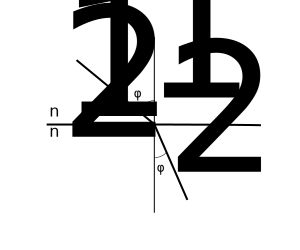
\includegraphics[width=0.5\textwidth]{img/refraction.pdf}
\caption{Преломление света}
\end{figure}

Очевидно, что при некотором угле падения синус соответствуюшего угла преломленния окажется больше единицы, что невозможно. В этом случае будет наблюдаться эффект полного внутреннего отражения. Это возможно только в случае $n_1 > n_2$

\begin{figure}[h!]
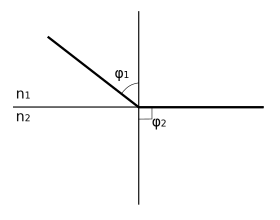
\includegraphics[width=0.5\textwidth]{img/refraction_full_inner.pdf}
\caption{Полное внутреннее отражение}
\end{figure}

\section{Планарные волноводы}

\begin{figure}[h!]
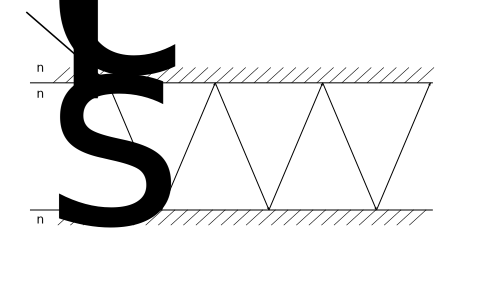
\includegraphics[width=0.9\textwidth]{img/planar_propagation.pdf}
\caption{Распространение света в волноводе}
\end{figure}

Планарный волновод - это структура из слоев с тремя разными показателями преломления с соотношением $n_f > n_s > n_c$ С точки зрения геометрической оптики, свет, попадая в волновод, испытывает ПВО последовательно от обеих границ и оказывается заключен в волноводной среде и рапространяется вдоль нее с максимальной эффективностью. Найдем распределение поля электромагнитных волн в волноводе из уравнений Максвелла \cite{adams}:

\begin{equation}
 	\nabla\times \mathbf{H} = -n_j^2\epsilon_0 \frac{d\mathbf{E}}{dt},
 	\label{makswell_1}
\end{equation}
\begin{equation}
	\nabla\times \mathbf{E} = -\mu_0\frac{d\mathbf{H}}{dt},
  	\label{makswell_2}
\end{equation}
\begin{equation}
 	\nabla\cdot \mathbf{E} = 0,
 	\label{makswell_3}
\end{equation}
\begin{equation}
 	\nabla\cdot \mathbf{H} = 0.
 	\label{makswell_4} 
\end{equation}

Подставив в уравнение (\ref{makswell_2}) величину $H$ из уравнения (\ref{makswell_1}) и применив оператор дивергенции, получим:

\begin{equation}
	\nabla^2\mathbf{E} = -\mu_0\epsilon_0 n_j^2 \frac{d^2\mathbf{E}}{dt^2}.
\end{equation}

Предполагая искомое решение в виде $E \sim \exp(-i\omega t)$, получим волновое уравнение:

\begin{equation}
	\nabla^2\mathbf{E} + k^2 n_j^2 E = 0,
\end{equation}

где $k^2 = \omega^2\mu_0 \epsilon_0$. Учитывая, что планарный волновод не ограничен положительном и отрицательном направлениях по оси y, то распределение поля однородно, а производная обращается в нуль. Кроме того, допустим, что по координате z определяется как $\exp(i\beta z)$, где $\beta$ - постояннная распространения, то уравнение для каждой из областей волновода запишется так:

\begin{equation}
	\frac{\partial^2 E_3}{\partial x^2} -(\beta^2 - n_3^2 k^2)E_3 = 0
\end{equation}

\begin{equation}
	\frac{\partial^2 E_1}{\partial x^2} -(n_1^2 k^2 - \beta^2)E_1 = 0
\end{equation}

\begin{equation}
	\frac{\partial^2 E_2}{\partial x^2} -(\beta^2 - n_2^2 k^2)E_2 = 0
\end{equation}

Большая часть энергии моды должна быть сосредоточена в центральной области с показателем преломления $n_1$. Этому условию подойдет решение, осциллирующее в области 1 и затухающее за ее пределами в областях 2 и 3. Поэтому запишем распределение поля в виде:

\begin{equation}
	E_y =
	\begin{cases}
		Ae^{-rx}, &\text{если $x \geqslant 0$;}\\
		A\cos qx + B\sin qx, &\text{если $0 \geqslant x \geqslant -2a $;}\\
		(A\cos 2aq + B\sin 2aq)e^{p(x+2a)}, &\text{если $-2a \geqslant x$.}
	\end{cases}
\end{equation}

\section{Цилиндрические волноводы}
Наряду с волноводами прямоугольного сечения применяются также цилиндрические волноводы круглого сечения. Как правило, такие волноводы состоят из сердцевины с высоким показателем преломления и оболочки с меньшим показателем преломления. 

\begin{figure}[h!]
	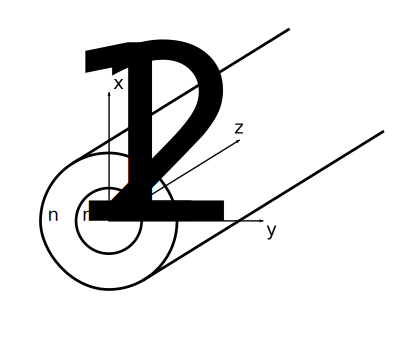
\includegraphics[width=0.7\textwidth]{img/cylinder_axes.pdf}
	\caption{Цилиндрический волновод}
\end{figure}

Для нахождения распределения поля воспользуемся волновым уравнением в цилнидрических координтатах:

\begin{equation}
	\frac{\partial^2\psi}{\partial r^2} + \frac{1}{r}\frac{\partial\psi}{\partial r}+\frac{1}{r^2}\frac{\partial^2\psi}{\partial\theta^2}+(n_j^2 k^2 - \beta^2)\psi = 0.
\end{equation}

Так как мы ищем решение с круговой симметрией, то общее решение будет иметь вид:

\begin{equation}
	\psi(r, \theta) = R(r)e^{i\nu\theta} \qquad (\nu = 0,1,2, ...),
\end{equation}

Где $\psi(r, \theta)$ - это продольная составляющая поля, $E_z$ или $H_z$. Подставляя решение в уравнение, получим:

\begin{equation}
	\frac{\partial^2 R}{\partial r^2} + \frac{1}{r}\frac{\partial R}{\partial r}+(n_j^2 k^2 - \beta^2 - \frac{\nu^2}{r^2}) = 0.
\end{equation}

Здесь возможны два варианта решения, для TE-мод, когда $E_z = 0$ и TM ($H_z = 0$). Найдем решение для TE-моды, в случае TM, уравнение решается аналогично

\begin{equation}
	H_z = H_0 J_v (\frac{ur}{a}),
\end{equation}

где $J_v$ - функция Бесселя, $\frac{u}{a} = \sqrt{k^2 n_j^2 - \beta^2}$